\documentclass{beamer}

\usepackage{tikz}
\usetikzlibrary{matrix}

%\usepackage{tieto}
\usetheme{Warsaw}

\title{Inside-Out: STL}
\subtitle{How to use it wisely?}
\author{Jadwiga Pokorska}
\institute{TietoEvry}
\date{26.02.2020}

\begin{document}
    %\usebackgroundtemplate{\includegraphics[width=\paperwidth,height=\paperheight,keepaspectratio]{Tieto_title.jpg}}

\begin{frame}
\titlepage
\end{frame}

\begin{frame}
\frametitle{Presentation plan}
\tableofcontents
\end{frame}

\section{Introduction}

\subsection{Time complexity}
\begin{frame}
    \frametitle{Time complexity}
    \begin{block}{Purpose}
    Time complexity is a tool to measure the efficiency of our algorithm.
    \end{block}

    \pause
    Usually defined with \textit{big-O} notation:
    \begin{itemize}
        \item $O(N)$,
        \item $O(N^2)$,
        \item $O(\log N)$,
        \item $O(N \cdot \log N)$,
        \item $O(\sqrt N)$,
    \end{itemize}
\end{frame}


\begin{frame}
    \frametitle{Task: find not paired item}
    \begin{block}{Task}
        Given an array of integers, find the only number that does \textbf{not}
        have a pair.
    \end{block}

    \pause
    \begin{example}
    For array $[2, 3, 7, 7, 2, 3, 2]$ the answer is $2$.
    \end{example}
\end{frame}

\begin{frame}[fragile]
    \frametitle{Task: find not paired item}
    \begin{verbatim}
int f(const vector<int>& t) {
    for (int selected_item : t) {
        int cnt = 0;
        for (int item : t)
            if (item == selected_item)
                cnt++;
        if (cnt % 2 == 1)
            return selected_item;
    }
    throw "All items have pairs!";
}\end{verbatim}

    \begin{block}{}
    What is the time complexity? \pause \textcolor{red}{$O(N^2)$}
    \end{block}
\end{frame}

\begin{frame}[fragile]
    \frametitle{Task: find not paired item}
    \small
    \begin{verbatim}
int f(const vector<int>& t) {
    std::sort(t.begin(), t.end());
    int cnt = 0, prev = -1;
    for (int i = 0; i < t.size(); ++i) {
        if (prev == t[i]) cnt++;
        else {
            if (cnt % 2 == 1) return prev;
            prev = t[i];
            cnt = 0;
        }
    }
    if (cnt % 2 == 1) return prev;
    throw "All items have pairs!";
}\end{verbatim}

    \begin{block}{}
    What is the time complexity? \pause \textcolor{red}{$O(N \cdot \log N)$}
    \end{block}
\end{frame}

\begin{frame}[fragile]
    \frametitle{Task: find not paired item}
    \begin{verbatim}
int f(const vector<int>& t) {
    int result = 0;
    for (int item : t)
        result ^= item;
    if (result > 0)
        return result;
    throw "All items have pairs!";
}\end{verbatim}

    \begin{block}{}
    What is the time complexity? \pause \textcolor{red}{$O(N)$}
    \end{block}
\end{frame}

\subsection{Vector}

\begin{frame}
    \frametitle{Vector - time complexity}
    Where do I find the information about the time complexity?
    \pause
    \textcolor{red}{Documentation!}

    \centering
    \includegraphics[width=8cm]{vector.png}
\end{frame}

\begin{frame}
    \frametitle{Vector - time complexity}
    \includegraphics[width=11cm]{vector_erase.png}
\end{frame}

\begin{frame}
    \frametitle{Vector - internal implementation}

    TODO: make piktures showing inserting elements (with resizing and copying).

    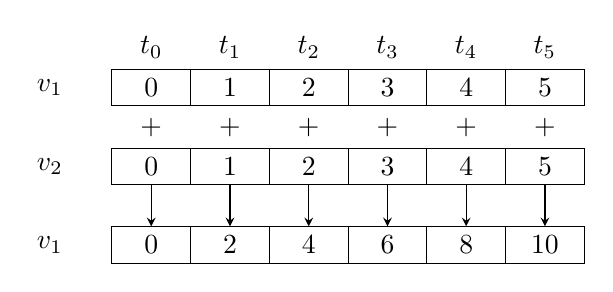
\begin{tikzpicture}
    \foreach \v [count=\y] in {1,2,1}{
  \node [left] at (0,-\y) {$v_\v$};
  \foreach \i [count=\x, evaluate={\j=int(\i+\i);}] in {0,...,5}{
     \node [minimum width=1cm,draw] (cell-\y-\x) at (\x,-\y) {\ifcase\y\or\i\or\i\or\j\fi};
     \ifcase\y
     \or
       \node [above=.25cm] at (\x,-\y) {$t_\i$};
     \or
       \node [above=.25cm] at (\x,-\y) {$+$};
     \else
       \draw [-stealth] (cell-2-\x) -- (cell-3-\x);
     \fi
  }
}
    \end{tikzpicture}
\end{frame}

\subsection{Sort?}

\section{Balanced trees}

\subsection{BST}

\begin{frame}
    \frametitle{}
    TODO.
\end{frame}

\subsection{AVL / Red-Black Tree}

\begin{frame}
    \frametitle{}
    TODO.
\end{frame}

\section{Hash tables}

\begin{frame}
    \frametitle{}
    What is it?
\end{frame}

\subsection{Hash table of integers}

\begin{frame}
    \frametitle{}
\end{frame}

\subsection{Hashing, perfect hashing, 2-universal hashing function families \dots}

\end{document}
